\scanpage{93}
\mspage{92}
En d'autres termes, on trouve un isom.
\inserted{de $\pi$-groupoïdes}
\[
(15)\qquad C'_{\unsure{\xi}}\simeq\mathcal E(E_{\unsure{\xi}})
\]
avec les notations introduites plus haut,
où $E_{\unsure{\xi}}$ est le $\mu$-torseur image inverse de
$\unsure{\xi}\in E_0=\operatorname{Ob}C$ par $E\longrightarrow E_0=E/\mu$.

De façon générale, étant donnée une
extension \inserted{centrale} de groupes \deleted{commutatifs} $\mathcal E$
(13), on appelle $(\pi,\unsure{\mu})$-\uline{fibration \inserted{(stricte)} de groupoïdes}
\uline{subordonnée} à l'extension (13), un
hom de groupoïdes
\[
(16)\qquad f:C'\longrightarrow C
\]
muni

$2^\circ)$ D'une op. \inserted{(externe)} de $\mu$ sur $C'$,
\deleted{de façon} \inserted{compatible avec les $\pi$-opérations internes}

$1^\circ)$ D'une op. (interne) de $\pi$ sur $C'$, i.e.
d'un hom
\[
\pi\longrightarrow\operatorname{Aut}(\operatorname{id}_{C'})
\]
satisfaisant les conditions suivantes
\margin{\figure{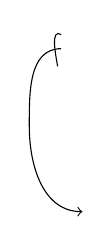
\begin{tikzpicture}[x=.45cm,y=.45cm]
\draw[->] (.9,4.6) to[out=180,in=90] (0,2.4) to[out=-90,in=180] (1.5,0);
\draw (.9,5) to[out=150,in=100] (.8,4.1);
\end{tikzpicture}}}

a) La structure $1^\circ)$ fait de $f$ une $\pi$-fibration
stricte, en particulier on a exactitude des suites
\unsure{(3)}, et bijectivité de $\pi_0(f)$
[$+$ surjectivité de $f_0$
sur les objets, qu'on \unsure{doit préciser}]
